\documentclass[conference]{IEEEtran}

\usepackage{graphicx}
\usepackage{url}
\usepackage{framed}
\usepackage{enumitem}
\usepackage{varwidth}
\usepackage{float}
\usepackage{subcaption}
\usepackage{balance}

\newcommand{\todo}[1]{ \textbf{#1} }
\newcommand{\quotes}[1]{\textit{``#1''}}
\newcommand{\code}[1]{\colorbox{light-gray}{\texttt{#1}}}
% correct bad hyphenation here
\hyphenation{op-tical net-works semi-conduc-tor}


\begin{document}

\title{How do Scratch Programmers Name Variables and Procedures?}

% author names and affiliations
% use a multiple column layout for up to three different
% affiliations
\author{\IEEEauthorblockN{Alaaeddin Swidan}
\IEEEauthorblockA{Delft University of Technology\\
The Netherlands\\
Email: alaaeddin.swidan@tudelft.nl}
\and
\IEEEauthorblockN{Alexander	Serebrenik}
\IEEEauthorblockA{Eindhoven University of Technology\\
	The Netherlands\\
	Email: a.serebrenik@tue.nl}
\and
\IEEEauthorblockN{Felienne Hermans}
\IEEEauthorblockA{Delft University of Technology\\
	The Netherlands\\
	Email: f.f.j.hermans@tudelft.nl}
}

% make the title area
\maketitle

% As a general rule, do not put math, special symbols or citations
% in the abstract
\begin{abstract}
Research shows the importance of selecting good names to identifiers in software code: more meaningful names improve readability. In particular, several guidelines encourage long and descriptive variable names.
A recent study analyzed the use of variable names in five programming languages, focusing on single-letter variable names, because of the apparent contradiction between their frequent use and the fact that these variables violate the aforementioned guidelines.

In this paper, we analyze variables in Scratch, a popular block-based language aimed at children. We start by replicating the above single-letter study for Scratch. We augment this study by analyzing single-letter procedure names, and by investigating the use of Scratch specific naming patterns: spaces in variable names, numerics as variables and textual labels in procedure names.

The results of our analysis show that Scratch programmers often prefer longer identifier names than developers in other languages, while Scratch procedure names have even longer names than Scratch variables. For the single-letter variables, the most recurring names are $x$, $y$ and $i$. Single-letter procedures are less popular, but show more tendency to be in upper case. When compared to the other programming languages, the usage of single uppercase letters in Scratch variables seems to be similar to the pattern found in Perl, while for the lowercase letters---to the pattern found in Java.
Concerning Scratch specific features, 44\% of the unique variable names and 34\% of the projects in the dataset include at least one space. The usage of textual string between parameters appears as not common, however textual patterns used imply an influence from textual languages, for example by using brackets.

The naming patterns found give an indication that Scratch programmers may incur difficulties when transiting to the use of mainstream textual programming languages. Those languages restrict the use of spaces in identifiers and more often divert into short and single-letter names---tendencies opposite to the naming preferences in Scratch.  
\end{abstract}

\IEEEpeerreviewmaketitle

\section{Introduction}
The naming of identifiers in the source code has been extensively studied (see, e.g., recent studies of this subject \cite{AmanASK15,AvidanF17,Beniamini,ButlerWYS10,HofmeisterSH17,LunguK13,ScannielloR13,TramontanaRS14}).
Still, the impact of the variable name choice on code readability and maintainability is controversial, as witnessed, e.g., by recent studies of Beniamini et al.~\cite{Beniamini} and Hofmeister et al.~\cite{HofmeisterSH17} reaching contradictory conclusions.

Furthermore, many computer science and programming curricula focus on the programming concepts and the syntax of the languages as opposed to practices in naming variables and identifiers. 
Indeed, while ``meaningful variable names'' are advocated by some teachers~\cite{Kato2016, hermans_aivaloglou} and practitioners~\cite{Rother} neither the ACM Curriculum Guidelines for Undergraduate Programs in Computer Science\footnote{\url{http://www.acm.org/education/CS2013-final-report.pdf}} nor the Curriculum Guidelines for Undergraduate Degree Programs in Software Engineering\footnote{\url{http://www.acm.org/binaries/content/assets/education/se2014.pdf}} discuss this topic.
In fact, as discussed by Raymond~\cite{Raymond} standard metasyntactic variables used in syntax examples are \quotes{foo} and \quotes{bar}.
The names of these identifiers are meaningless, and to some extent, they represent a refusal to name, suggesting the learner that naming is less important %, or irrelevant, 
to the programming task. 

%Recent studies have focused on the analysis of identifier naming in software code repositories, with a focus on single letter variables, since they are considered especially ambiguous. 

The goal of this paper is to \textbf{understand the patterns in variable and procedure naming in Scratch}. Scratch is a block-based visual language developed by MIT with the aim of helping young people learn the basic concepts of programming and collaboration. 
Scratch has recently become very popular among school-age children and in several countries has been introduced as part of the school curriculum as a means to teach programming~\cite{vanZyl,SaezLopez}.
Moreover, the overall popularity of Scratch is witnessed by Scratch being currently rated 19 in the TIOBE index\footnote{\url{https://www.tiobe.com/tiobe-index/}}, topping such languages as Lua, Scala and Groovy and since early 2014 exhibiting an increasing trend shown in Fig.~\ref{fig:tiobe}.
\begin{figure}
  \begin{center}
  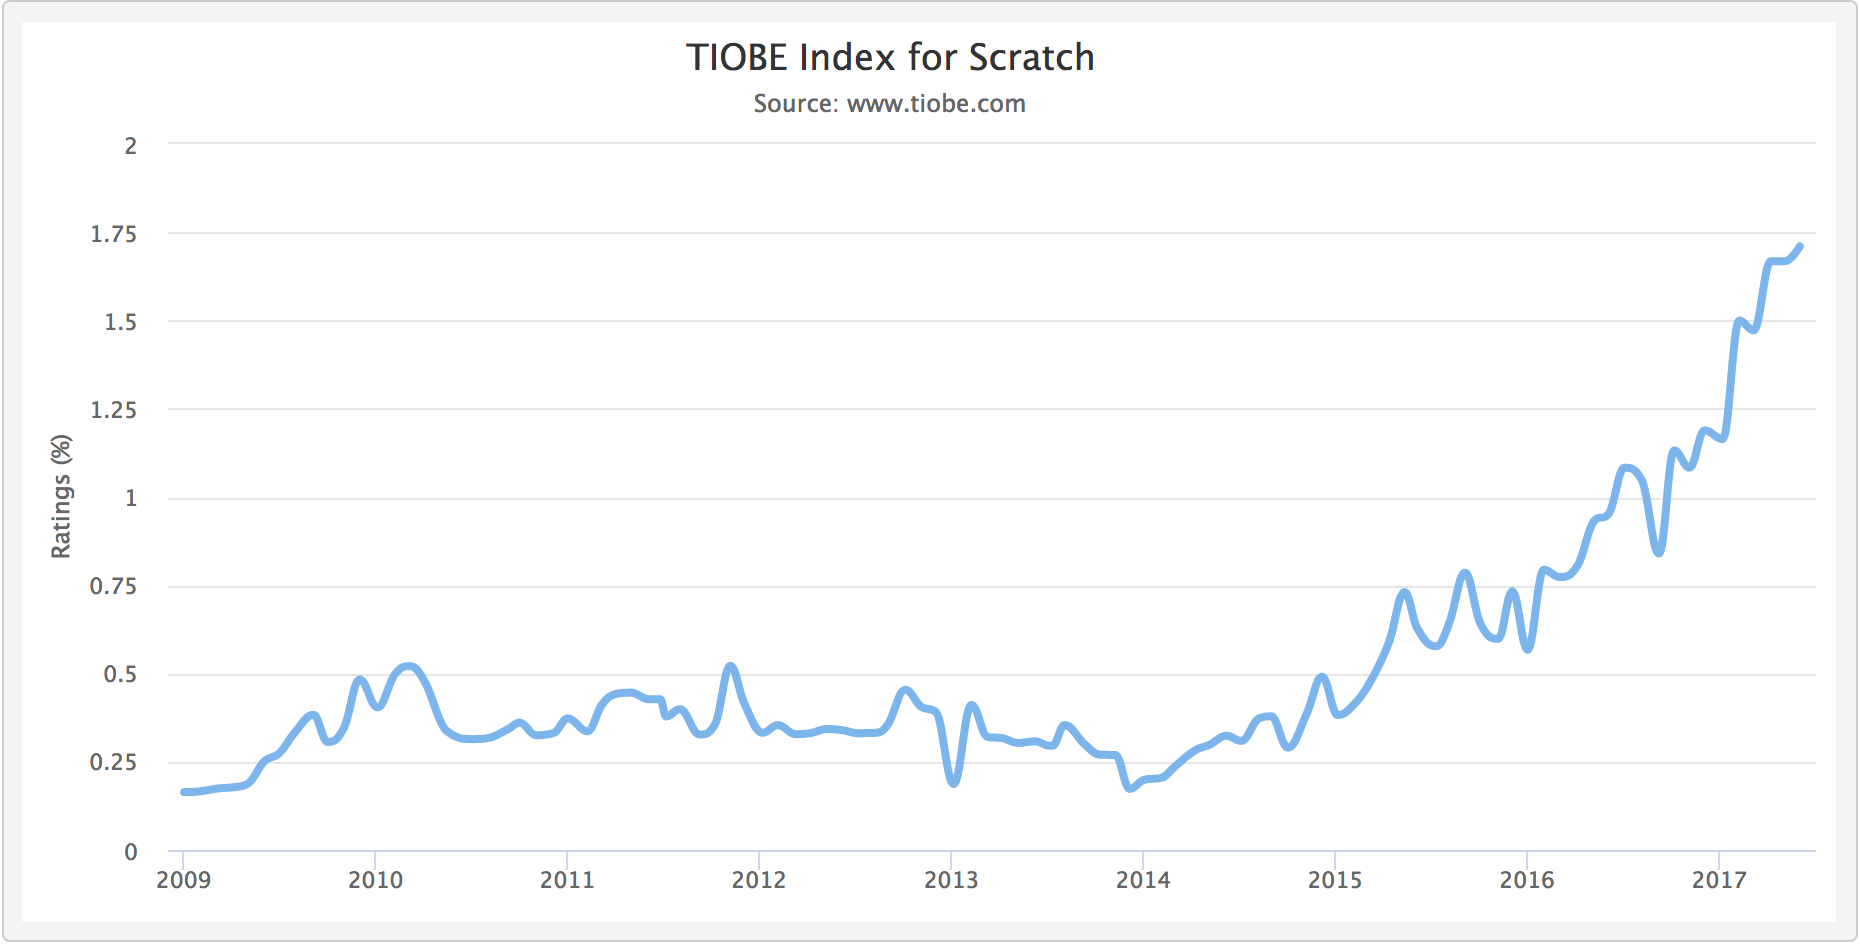
\includegraphics[scale=0.25]{fig/tiobe}
  \caption{TIOBE Programming Community index: evolution of the popularity of Scratch}
  \label{fig:tiobe}
  \end{center}
\end{figure} 

\begin{figure}[tb]
	\begin{center}
``		\includegraphics[width=0.9\columnwidth]{fig/Scratch_users}
		\caption{Age distribution of Scratch users at the time of registration according to Scratch statistics web-page}
		\label{fig:Scratch_users}
	\end{center}
\end{figure} 

Scratch programming materials too do not focus on naming. For example, the Creative Computing Learner Workbook created by the ScratchEd group at Harvard does not explain how to select good names for procedures and variables \footnote{\url{http://scratched.gse.harvard.edu/guide/files/CreativeComputing20140820_LearnerWorkbook.pdf}}. It is therefore interesting to explore the naming habits of Scratch programmers. And there are other reasons why understanding the naming practices in the Scratch community is important. First, it is important for the Scratch community itself as bad naming practices can easily propagate from one program to another through `remixing'~\cite{Hill:Monroy-Hernandez,Davis:Kafai:Vasudevan:Lee}, code sharing practice similar to GitHub forking.
Second, it is important for researchers. Software engineering researchers can learn how to support novice programmers, taking their first steps in programming. As shown in Fig.~\ref{fig:Scratch_users}, 51\% of Scratch programmers are aged between 10 and 15 at the time of registration according to the statistics provided by Scratch\footnote{\url{https://Scratch.mit.edu/statistics/}}. Therefore, researchers on software engineering education can obtain insights in how to define naming guidelines for educational materials, and analyzing the differences between Scratch and textual languages can help in supporting the transition from visual languages to textual ones~\cite{Dann,Matsuzawa}. 

We start by a \textbf{general discussion of naming practices} in Scratch and analyze the previously published collection of 250,000 Scratch projects~\cite{Aivaloglou2016HowKC}. 
We replicate two studies from a recent paper by Beniamini et al.~\cite{Beniamini}.
Similarly to Beniamini et al. we investigate the distribution of the lengths of variable names and study popularity of single-letter variable names such as $i$ and $x$.
As opposed to Beniamini et al. who focused on variable naming in five mainstream programming languages we focus on Scratch.
Furthermore, while Beniamini et al. solely focused on the names of the variables, we repeat their study for procedure names as well.

\begin{framed}
Variable names in Scratch range mostly between 4 and 10 characters. While procedure names tend to be longer. 
For the single-letter variables, the most commonly used names are $x$, $y$ and $i$, procedures---$a$, $y$ and $r$. 
When compared to the other programming languages, we observe that single-letter variable names are less common in Scratch and that overall Scratch variables have longer names. 
The usage of single uppercase letters is similar to the pattern found in Perl, for the lowercase---to the pattern found in Java.
\end{framed}

%\todo{"range between 4 and 14 characters" -> not true, 1 also exists? discuss tomorrow.}\todo{yes, but they still ``tend'' to rand between 4 and 14, no ideas where do the numbers come from. Better: ``50\% of the variables have length between 5 and 11 characters''? Q1: 5, Q3: 11. }
%while procedure names tend to be longer and commonly range between 4 and 14 characters. 


Next we focus on \textbf{Scratch-specific features in naming identifiers}. Scratch supports a number of less commonly used naming features, for example spaces may be used in names e.g., a variable \emph{max i} and integers and even floating point numbers can be used as variable names e.g., a variable named \emph{6} or \emph{3.14159}. Finally, Scratch allows for textual labels in between parameters. For example a method for printing the first $n$ letters from a string $s$ could be called ``printnof($n$,$s$)'' in a textual language. Scratch allows for this too, however, one can also define a procedure called ``say $n$ characters from text $s$", as shown in Fig. \ref{fig:procedures}. 
This feature does exist in textual languages too---most notable in SmallTalk---but is not commonly found in most mainstream languages. 

Investigating the use of these Scratch-specific naming patterns is interesting to understand their role in novice programming. If they are popular among Scratch programmers, this might be because they ease novice programming, and that means one could even advocate that these features should be integrated in the textual programming languages, if only to ease the transition for the block-based languages programmers.

\begin{framed}
 Spaces in variable names are common: 34\% of projects use this feature. 
 Numeric values as identifiers are rarely used, and mostly represent constants or parts of the data structure.
 The usage of textual string between parameters is not so common, however, textual patterns used imply an inference from textual languages, e.g., by using brackets. 
\end{framed}

\section{Related work}
Naming identifiers in software code has been studied extensively in the past decades~\cite{AmanASK15,AnquetilL98,AvidanF17,Beniamini,ButlerWYS10,CaprileT00,HofmeisterSH17,LawrieMFB07,LunguK13,ScannielloR13,TakangGM96,Teasley,TramontanaRS14}. 
In practice, identifiers constitute a major part of the source code: e.g., Dei{\ss}enb{\"o}ck and Pizka found that in Eclipse 3.0M7 which is tantamount to 2 MLoC, 33\% of the tokens and 72\% of characters correspond to identifiers~\cite{Deissenbock}. 

For a human reading code, it is crucial to the understanding of code to also understand what the identifiers mean. As such, several studies have investigated the link between identifier naming and code readability and comprehension~\cite{AvidanF17,HofmeisterSH17,LawrieMFB07,TakangGM96,Teasley} or identifier naming and externally observable aspects of the software development process that are expected to be affected by comprehension such as change-proneness~\cite{AmanASK15}, quality~\cite{ButlerWYS10,LunguK13} and presence of faults~\cite{ScannielloR13,TramontanaRS14}.
Caprile and Tonella~\cite{CaprileTonella} have observed that names of C functions consist of on average of 2.04--3.36 words, often verbs expressing action, while Caracciolo et al. observed that most method names in Java and Smalltalk also tend to consist of several words but rarely more than five words~\cite{Caracciolo}.
%The comprehension is not a target in its own; the true reason is that better comprehension lets the developers perform maintenance tasks more effectively and efficiently.
%But what is a good naming approach? 
%It is out of this paper's scope to explore the various recommendations of good identifier naming. 
%However, it is worth to mention that there are different perspectives on what a good name is. 
%Some researchers emphasize the usage of actual and complete words from a dictionary, or known abbreviations, which reflect the context of the program's purpose. 
%Others argue that consistency in naming style is the most important. 
%The usage of single-letter identifiers attracts much attention in research. 
%For programmers, it is tempting to choose single-letter identifiers for quicker code writing that involves less mental load on the choice of a name. 
%Additionally, single-letter named variables such as \quotes{i} or \quotes{j} have become almost a standard choice for index values when coding loops. 
%Research has shown however that shorter identifier names are longer to comprehend, and the length of a variable should reflect its scope. 
%
%Despite the agreement on the importance of identifier names, and efforts to introduce naming guidelines and additional tools to help the programmer choose better names, developers find giving appropriate names to identifiers as a difficult task. In the end, it is the decision of the individual writing the code, and many factors may contribute to that decision. One area to consider here is the computer science and in particular programming education. There seems to be a great focus on the programming concepts, while less to zero attention is given to beautifying the code. For example, the usage of the identifier names \quotes{foo} and \quotes{bar} is prevalent in code examples. These names have no real meaning, and the student cannot link them to what the code does.  
%
%We are inspired by the work done by Beniamini et al.~\cite{Beniamini} where they explored the single-letter naming for multiple software repositories from different programming languages. It is important for the software community to understand the patterns in which software developers apply naming to identifiers. We argue that this understanding can improve the quality of the guidelines and introduce research-supported tools that meet the needs of the programmers. For this sake, we believe it is even more important to focus on the novice programmers, students, and learners. For these future developers, the usage of a particular naming pattern in this level forms a (mis)conception that could move along with them to other programming languages and future careers. 

Going beyond the discussion of whether variable names should be shorter or longer, Arnaoudova et al.~\cite{ArnaoudovaPAG13,ArnaoudovaPA16} have studied linguistic anti-patterns, ``recurring poor practices in the naming, documentation, and choice of identifiers in the implementation of an entity'' such as discrepancies between the behavior implied by the identifier (e.g., {\sc INCLUDE\_NAME\_DEFAULT} in the Cocoon Apache project) and the corresponding comment (``Configuration default exclude pattern''), or between the identifier and commonly applied guidelines (e.g., getter that does not only access fields). 
In the educational setting Glassman et al. propose Foobaz, a tool giving semi-automatic feedback on student variable names based on the values the variable can take during the execution and limited input from the teacher~\cite{Glassman}.
% elementary and high 
While visual languages such as Scratch, Sqeak and Alice recently become a favorable choice for schools as an introduction to programming~\cite{Matsuzawa}, the lion's share of the previous work on identifier naming has focused on textual languages.
Notable exception is the recent work of Moreno and Robles~\cite{MoreonoRobles}: Moreno and Robles have observed that Scratch programmers often do not change the sprite names that were automatically generated by the environment. 
van Zyl et al. have observed that one of the interviewed school teachers working with Scratch has taught the students to integrate variable types in their names, e.g., `S' for Strings~\cite{vanZyl}. Finally, Hermans and Aivaloglou encouraged the students in Scratch MOOC to choose meaningful names and to avoid keeping default ones~\cite{hermans_aivaloglou}. 
% These block-based languages allow the user to create and assign their identifiers for variables and blocks. By studying these identifiers, we can understand better how novice programmers apply standard and language-specific naming, and how it compares to other textual based languages previously explored in the literature. 

\section{Relevant Scratch Concepts}
\label{sec:Scratch}
We briefly introduce several core features of Scratch required for understanding the reminder of the paper. 
Interested readers are referred to \cite{brennan_creative_2014} for an extensive overview.  

Scratch is a block-based programming language aimed at children, developed by MIT. Scratch can be used to create games and interactive animations, and is available both as a stand-alone application and as a web application. Figure~\ref{fig:ui} shows the Scratch user interface in the Chrome browser.

\subsubsection{Sprites}
Scratch code is organized into `sprites': two-dimensional pictures that each have their own source code. Scratch allows users to bring their sprites to life in various ways, for example by moving them in the plane, having them say or think words or sentences via text balloons, but also by having them make sounds, grow, shrink and switch costumes. 

The Scratch program in Fig.~\ref{fig:ui} consists of one sprite, the cat, which is Scratch's default sprite and logo\footnote{\url{https://Scratch.mit.edu/projects/97086781/}}. The code in the sprite will cause the cat to jump up, say ``hello'', and come back down, when the green flag is clicked, and to make the `meow' sound when the space bar is pressed.

\begin{figure}
  \begin{center}
  \includegraphics[width=\columnwidth]{fig/ui.png}
  \caption{The Scratch UI consisting of the `cat' sprite on the left, the toolbox with available blocks in the category `motion' in the middle and the code associated with the sprite on the right.}
  \label{fig:ui}
  \end{center}
\end{figure} 

%\subsection{Events}
%Scratch is \emph{event-driven}: all motions, sounds and changes in the looks of sprites are initiated by events. The canonical event is the `when Green Flag clicked', activated by clicking the green flag at the top of the user interface. In addition to the green flag, there are a number of other events possible, including key presses, mouse clicks and input from a computer's microphone or webcam. In the Scratch code in Figure \ref{fig:ui} there are two events: `when Green Flag clicked' and `when space key pressed'

\subsubsection{Scripts}
Source code within sprites is organized in scripts: a script always starts with an event, followed by a number of blocks. The Scratch code in Fig.~\ref{fig:ui} has two distinct scripts, one started by clicking on the green flag and one by pressing the space bar. It is possible for a single sprite to have multiple scripts initiated by the same event. In that case, all scripts will be executed simultaneously. 

%\subsection{Remixing}


\subsubsection{Variables}
Like most textual languages, Scratch programmers can use variables. Variables are untyped, but have to be `declared' through the Scratch user interface, shown in Fig.~\ref{fig:ui-vars}. This figure also shows that, contrary to most programming languages, variable names in Scratch may contain spaces.

\begin{figure}
  \begin{center}
  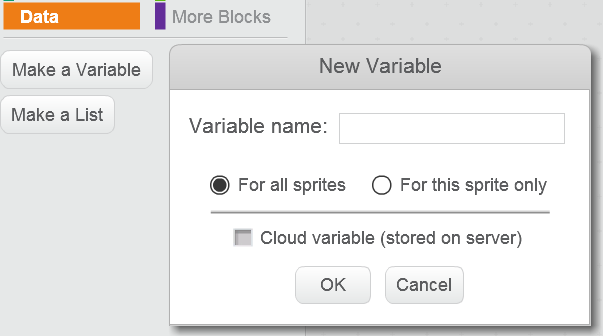
\includegraphics[scale=0.45]{fig/ui-vars.png}
  \caption{The Scratch user interface to create a variable}
  \label{fig:ui-vars}
  \end{center}
\end{figure} 

\subsubsection{Procedures} \label {sec:Scratch_func}
Scratch allows programmers to create their own blocks, called procedures. They can have input parameters, and labels in between. Procedures are created with an interface similar to the one to create variables. Figure~\ref{fig:procedures} shows the definition and the invocation of a procedure in Scratch.

\begin{figure}
  \begin{center}
  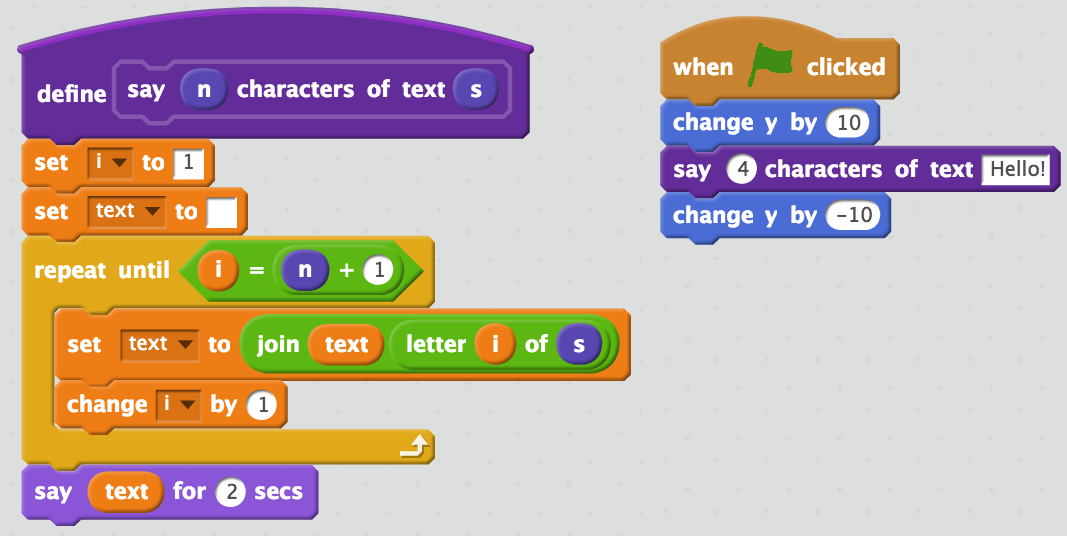
\includegraphics[scale=0.28]{fig/procedures2.png}
  \caption{Scratch code to define and invoke a procedure}
  \label{fig:procedures}
  \end{center}
\end{figure} 


\section{Research design and dataset}
\subsection{Overall design}
\label{sec:design}
The goal of this paper is to compare naming practices of the Scratch programmers to those of the developers in the mainstream programming languages. To that end, we start by partially replicating the recent work of Beniamini et al. on single-letter variables in Java, C, PHP, Perl and JavaScript~\cite{Beniamini}. 
In terms of the classification of Shull et al.~\cite{Shull2008} we perform a dependent replication of the studies summarized in Fig.~1 and 2 of the original work.  
Inherently, the programming language is the only factor we vary when compared to the original study. 
However, as opposed to the data in the original study, Scratch programs are not available on GitHub. 
Hence, we use the dataset previously scraped and processed by Aivaloglou and Hermans~\cite{Aivaloglou2016HowKC}. 
We report on the results of these replications in Sections~\ref{res:var:length} and \ref{res:var:names}.
%
Furthermore, we perform another dependent replication of the same studies by considering Scratch procedures rather than variables (Section~\ref{res:proc}).

%%% TO REMOVE HERE IF THE TYPES ARE TO BE DROPPED
Next, we perform a conceptual replication of the study of the single-letter variable types of Beniamini et al.~\cite{Beniamini}. 
The original study has conducted a survey to understand the type-related user perceptions, with questions such as \emph{``what type would you consider for a variable called ...?''}. We however focus on the types as used in the program. 
We opt for types as being used as opposed to as being perceived due to limited programming experience of the intended Scratch programmers.
Scratch is meant for people taking their first steps in programming, such as school-age students and we do not expect them to have established  perceptions on data types of single-letters variables. 
As opposed to our work, in the original study however, 30\% of survey respondents claim a 10-years experience in programming, while  23\% have programming knowledge in six different languages or more~\cite{Beniamini}. 
Furthermore, we study types as used as opposed to types as defined, since Scratch does not have a concept of an explicit variable type.
However, we can deduce the variable types from assignments involving those variables. 
For example, the two variables in Fig.~\ref{fig:types} represent a string and an integer respectively. 
Results of this conceptual replication are presented in Section~\ref{res:types}.

\begin{figure}
	\begin{center}
		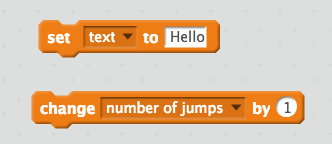
\includegraphics[width=5cm]{fig/types}
		\caption{Two variables, one of type string and one of type integer}
		\label{fig:types}
	\end{center}
\end{figure} 
%%%%% END TYPES

Finally, in Section~\ref{res:Scratch:specific} we report on the ways Scratch developers employ Scratch-specific naming practices such as spaces in variable names, numeric values as variables and the use of textual labels in between parameters.

\subsection{Dataset}
For this paper we use the dataset created by Aivaloglou and Hermans~\cite{Aivaloglou2016HowKC}, consisting of 250,000 Scratch projects scraped from the Scratch website in March 2016. 
From this dataset, we have selected the projects that use variables or procedures, which amount to 73,473 projects, 29\% of the Aivaloglou and Hermans's original dataset. 
Variables are used more often than procedures: 69,045 projects (27.6\%) use variables, while 17,605 use procedures (7\%). 
We used Python to process the original dataset and generate the graphs in this paper.

\subsection{Identifier Extraction}
To follow the steps of the replicated study, we collect the unique variable names used in the projects' scripts. 
Within the scripts we identify Scratch blocks that are used to assign a value to the variables, : e.g., ``Change \textit{variable} by \textit{value}" or ``Set \textit{variable} to \textit{value}". 
Variable names in Scratch are unique: once a variable is declared in a project, its name cannot be used to create another variable in the same project, even in a different scope, e.g., in a different sprite.  
%Therefore, counting occurrences of a particular variable name is the same as counting the projects where the variable is found. 

To determine the type of single-letter variables, we perform type inference on the parameter value assigned to each variable. 
The inference is performed via standard data type conversion of the value.
If the variable is accessed multiple times in a project with different data types, for example first as a string and then as an integer, both data types are counted.

For the procedure names, we follow a similar approach to the extraction of variable names. We extract the blocks used to call a particular procedure and then extract the name of the procedure, and count the number of projects in which a procedure name occurs. 

We note here that Scratch allows the user to create multiple procedures with the same exact name in the same sprite. It is not clear to us why the language would support such a feature.  We argue however that counting the procedure names once per project is an indication of the naming patterns used, and fits the needs of this study. For the presence of spaces in and numbers as variables we simply analyze the previously extracted variable names, while textual patterns in procedure names are detected from the extracted procedures' names.
We provide the Python code, input and output files for verification and replication purposes on a GitHub repository\footnote{\url{https://github.com/Felienne/ScratchVars}}.

\subsection{Data Analysis}
\label{sec:da}
%To augment the visual comparison of the data we conduct statistical analysis. 
Understanding differences in variable name lengths occurring between different programming languages requires comparison of multiple distributions. 
Such a comparison is traditionally performed as a two-step process consisting of (1) testing a global null hypothesis, that can be intuitively formulated as ``all distributions are the same'', using ANOVA or its non-parametric counterpart, the Kruskal-Wallis test, and (2) performing multiple pairwise comparisons of different distributions, testing specific subhypotheses such as ``distributions 2 and 4 are the same''. 
However, it has been observed that such a two-step approach can result in inconsistencies when either the global null hypothesis is rejected but none of the pairwise subhypotheses is rejected or vice versa~\cite{Gabriel}. 
Moreover, it has been suggested that the Wilcoxon-Mann-Whitney test, commonly used for subhypothesis testing, is not robust to unequal population variances, especially in the unequal sample size case~\cite{Zimmerman:Zumbo}
Therefore, one-step approaches have been sought.
We opt for one such approach, the $\widetilde{\mathbf{T}}$-procedure of Konietschke et al.~\cite{Konietschke:Hothorn:Brunner,Konietschke:nparcomp}. 
This procedure is robust against unequal population variances, respects transitivity, and has been successfully applied in empirical software engineering~\cite{VasilescuSGM14,VasilescuCS14,YuWYW16}.
In particular, we use the Tukey (all-pairs) contrasts to compare all distributions pairwise.

To understand differences and similarities between the distributions of single-letter variable names in different languages we represent each programming language as a 26-dimensional vector with the dimensions corresponding to `a', ..., `z'.
To eliminate sensitivity in the ways the distance matrix is computed we first calculate the cosine similarity between vectors and compare the mean similarity of a language to the remaining languages in the dataset, and then perform hierarchical clustering based on the Euclidean distance.

When comparing distributions of variable name lengths with the procedure name lengths, the $\widetilde{\mathbf{T}}$-procedure is not applicable.
Hence, we perform the Mann-Whitney-Wilcoxon test together with the two-sample test for the nonparametric Behrens-Fisher problem, i.e., test for
$H_0: p = 1/2$, where $p$ denotes the relative effect of the two independent samples~\cite{Neubert,Konietschke:nparcomp}.

For spaces use in variables' names we do two things: (i) To understand how much popular spaces are among all the names, we extract the space count per unique variable name. (ii) To understand the trend of using spaces across the dataset (multiple projects and multiple users), we extract per project the maximum space count in found in the project's variables. For the textual patterns in procedure names, we count the occurrence of each of the extracted token. 

 \section{Results}
This section presents an overview of our analysis of variable and procedure name use in the previously published Scratch dataset~\cite{Aivaloglou2016HowKC}. 
We start by replicating studies of Beniamini et al.~\cite{Beniamini} and proceed with investigating Scratch-specific features.

\subsection{Replication Studies}
Our first analyses are the replication studies regarding one letter variables.

\subsubsection{Variable Name Length}
\label{res:var:length}
The original study of Beniamini et al.~\cite{Beniamini} has concluded that the single-letter variable names \emph{``are approximately as common as other short lengths except in PHP''} and that \emph{``in C, Java, and Perl they make up 9--20\% of the names''}. 
Figure~\ref{fig:distribution_of_lengths} shows the distribution of lengths in the Scratch dataset. A closer look at the data reveals that the single-letter variables constitute ca. 4\% of all the variable names, i.e., less than the 9--20\% observed by Beniamini et al.
\begin{figure}[tb]
	\begin{center}
		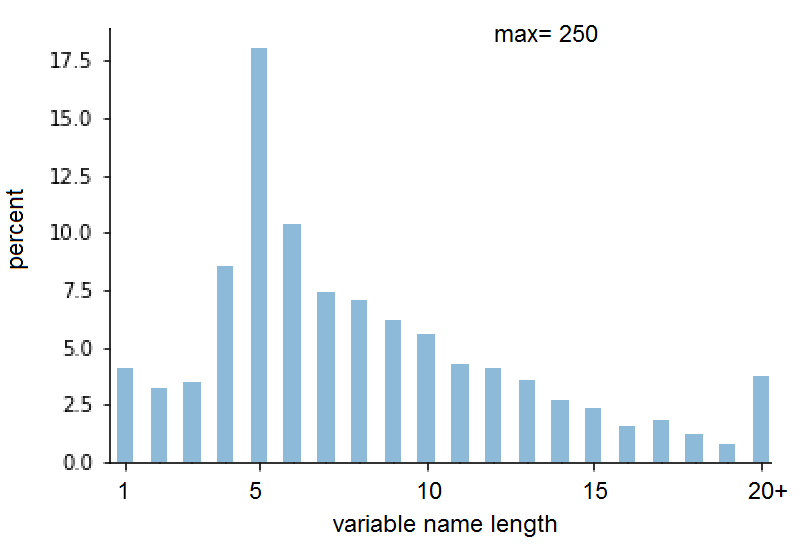
\includegraphics[scale=.3]{fig/project/distribution_var_name_length}
		\caption{The distribution of variable's name length in Scratch projects}
		\label{fig:distribution_of_lengths}
	\end{center}
\end{figure} 
Compared to the five programming languages in the study of Beniamin et. al., single-letter variables seem to be less common in Scratch, while the maximum length of a variable's name --250 characters-- is significantly larger. 
These \emph{Observation}s lead us to wonder whether overall the variable names in Scratch are longer than in other programming languages.
To this end, we apply the $\widetilde{\mathbf{T}}$-procedure described in Section~\ref{sec:da}. 
Statistical analysis reveals that variable names in Scratch indeed are longer than in the textual languages studied in Beniamini et. al.
Moreover, variable names in Java tend to be longer than those in PHP, variable names in  PHP than those in C, variable names in C than those in JavaScript and finally variable names in JavaScript longer than those in Perl. In all cases $p$-values have been too small to be computed precisely.

\subsubsection{Single-letter Variable Names}
\label{res:var:names}
Further we investigate the case of single-letter variable names. For the previously studied programming languages, the authors in~\cite{Beniamini} highlight the following \emph{Observation}s about the single-letter usage: 

\begin{enumerate}[label=\emph{\alph*})]
\item The most commonly occurring single-letter variable name is $i$.
The authors attribute this to $i$ being commonly used as a loop counter. 
As opposed to the studied mainstream languages, loops are performed in Scratch using predefined blocks. 
As illustrated on Fig.~\ref{fig:loop_Scratchblocks}, the  two left-most blocks --forever and repeat 10-- do not require a variable to control the loop iterations. However, inside the loop the user will have no access to the built-in loop's iterator. When that is needed by the user, then the third block in Fig.~\ref{fig:loop_Scratchblocks} --repeat until-- can be used. To understand its use see Fig.~\ref{fig:procedures}. In summary,  because of the built-in language support to variable-free loops, we expect the usage of the variable name $i$ to be less common in Scratch. \label{single-letter-vars:i}

\item Apart from the popularity of $i$ the distribution is language-dependent. 
Since Scratch is quite different from the programming languages considered by Beniamini et al., we expect the distribution of the single-letter variable names in Scratch to be different to the distributions in those languages. 
Hence, we expect the \emph{similarity} between Scratch and the languages considered by Beniamini et al. to be lower than the \emph{similarity} between those five languages in Beniamini et. al. study. \label{single-letter-vars:similarity}

\item Finally, the authors observe that the lower case letters are used more frequently than the upper case letters. Since this is also the case for regular text in most natural languages as well, we expect the Scratch programs to follow the same pattern. \label{single-letter-vars:upercase:lowercase}
\end{enumerate}

\begin{figure}[h]
	\begin{center}
		\includegraphics[scale=0.48]{fig/loops_in_Scratch}
		\caption{Scratch blocks that are used to repeat specific actions}
		\label{fig:loop_Scratchblocks}
	\end{center}
\end{figure} 

\begin{figure}[h]
	\begin{center}
		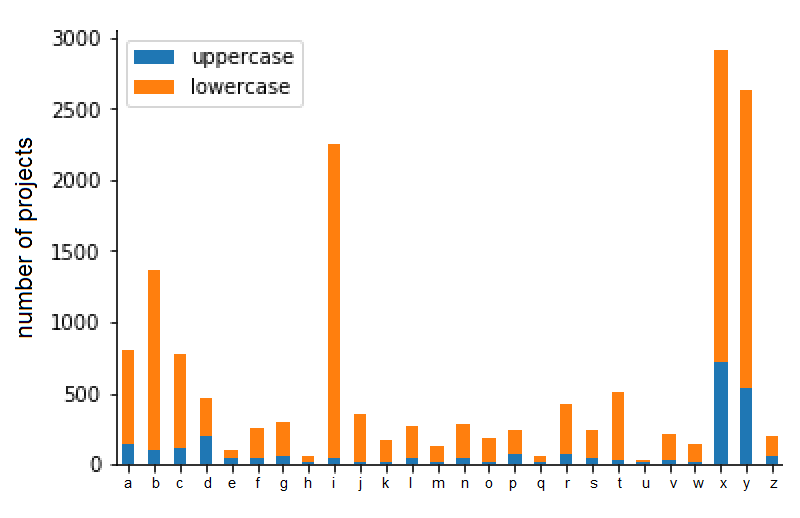
\includegraphics[width=0.95\columnwidth]{fig/project/varname_singleletter-project}
		\caption{A histogram of single-letter variables occurrences in Scratch projects }
		\label{fig:one_letter_occurrence}
	\end{center}
\end{figure} 
Figure~\ref{fig:one_letter_occurrence} shows the distribution of variables of one letter, in upper and lower case, in the Scratch dataset. 
Inspecting the data we observe that similarly to the previous study $i$ is the most commonly occurring variable. 
Hence, we conclude that \emph{contradicting our expectations} \emph{Observation}~\ref{single-letter-vars:i} above also holds for Scratch.
Furthermore, we observe that $x$ and $y$ are extremely popular in Scratch. 
This can be explained by the fact that $x$ and $y$ represent the coordinates of the sprites on the stage. They thus form the basis of moving sprites in the 2-D stage. There seems to be an agreement on this use among the developers of textual languages studied in Beniamini et. al. When they were surveyed about variable name interpretations, $x$ and $y$ were commonly interpreted as ``coordinates". In addition, built-in Scratch blocks often use $x$ and $y$ as shown in \figurename{~\ref{fig:xy_Scratchblocks}}. 
We conclude that Scratch programmers seem to be inspired by the Scratch language in naming their own variables.  

\begin{figure}[h]
	\begin{center}
		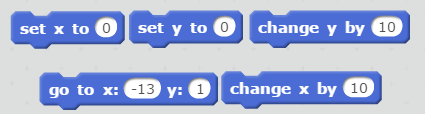
\includegraphics[scale=0.5]{fig/builtinblocks_xy}
		\caption{Some Scratch blocks that use built-in variables x and y}
		\label{fig:xy_Scratchblocks}
	\end{center}
\end{figure} 
Next we study the similarity of Scratch to the five programming languages in terms of frequency distribution of single-letter variable names.
Hence, we compare the mean cosine similarity of the twelve distributions (the five programming languages plus Scratch, considered for the uppercase and the lowercase letters).
The mean cosine similarity shows that the Scratch usage of the uppercase letters in the single-letter variable names is the most dissimilar among the
twelve distributions (0.39), while the way lowercase letters are used in Scratch quite similarly to the way letters are used in the five programming languages (0.62).
Hence, we claim that our expectation based on \emph{Observation}~\ref{single-letter-vars:similarity} has been confirmed for the uppercase letters and  rejected for the lowercase letters. 
Closer look at Fig.~\ref{fig:similarity_single_letter} shows that the usage of single uppercase letters is similar to the pattern found in Perl, for the lowercase---to the pattern found in Java.

Finally, Fig.~\ref{fig:one_letter_occurrence} clearly shows that the lowercase letters are much more often used as variable names than the uppercase letters, providing support for \emph{Observation}~\ref{single-letter-vars:upercase:lowercase}.
\begin{framed}
	Single-letter variable names are less common in Scratch than in other programming languages, and Scratch variables have longer names than variables in other programming languages.
\end{framed}

\begin{figure}[tb]
	\begin{center}
		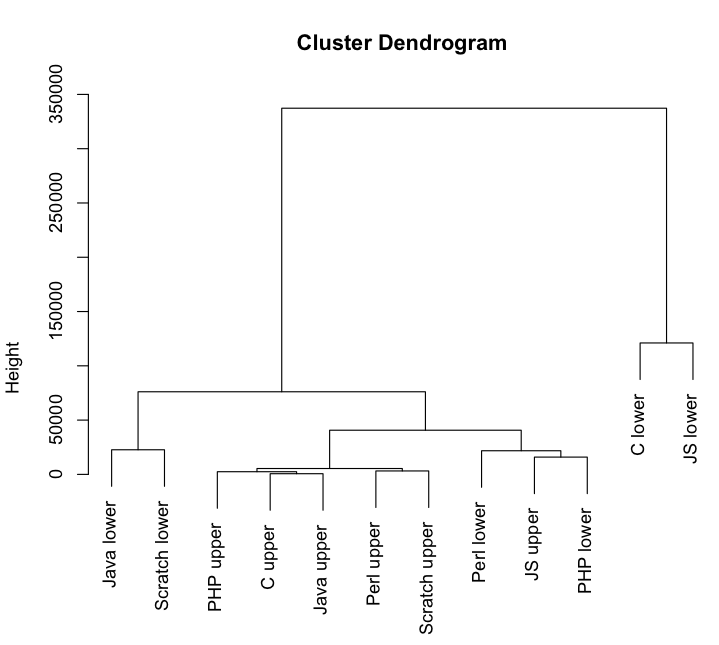
\includegraphics[width=\columnwidth]{fig/cluster_single_letter}
		\caption{A cluster dendrogram of Scratch compared to other programming languages for the single-letter pattern}
		\label{fig:similarity_single_letter}
	\end{center}
\end{figure} 


\subsubsection {Procedure Names}
\label{res:proc}
\begin{figure}[h]
	\begin{center}
		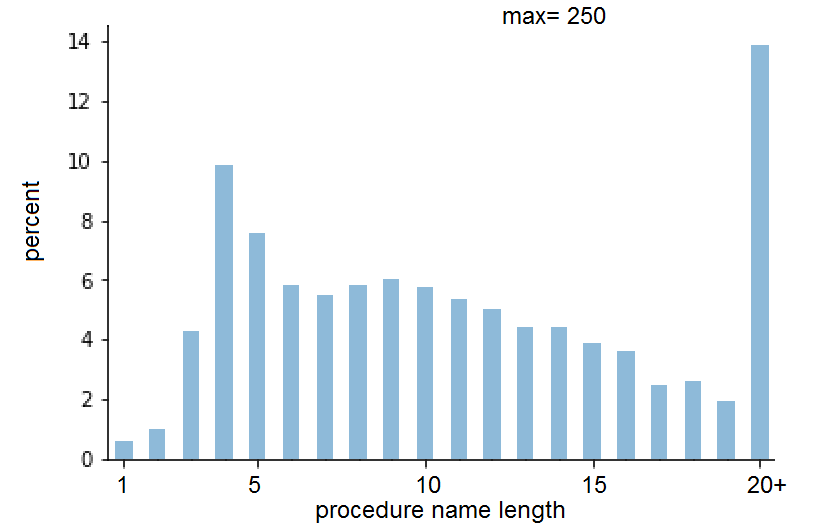
\includegraphics[scale=0.28]{fig/project/distribution_proc_name_length}
		\caption{The distribution of procedure's name length in Scratch projects}
		\label{fig:distribution_of_lengths_func}
	\end{center}
\end{figure} 

Going beyond the study of Beniamini, we additionally consider the naming of procedures in Scratch. 
For a detailed explanation of procedures in Scratch see Section~\ref{sec:Scratch_func} and Fig.~\ref{fig:procedures}. Figure~\ref{fig:distribution_of_lengths_func} shows the distribution of the procedure names length in the Scratch dataset. 
By inspecting this figure we observe that \emph{the procedure names tend to be longer compared to Scratch variable names}.
Indeed, the two-sample test for the nonparametric Behrens-Fisher problem estimates the relative effect of the two samples (procedure name lengths vs. variable name lengths) as $0.149$ (with the $p$-value being too small to be computed precisely), i.e., it indicates that the procedure names' lengths tends to be larger than the lengths of the variable names. 
This \emph{Observation} is additionally confirmed by the Mann-Whitney-Wilcoxon test (the $p$-value is too small to be computed precisely).
Short procedure names are not common, they are even less common than variable names: single-letter procedure names compose less than 1\% of the extracted names, less than 4.9\% observed for Scratch variables and 9--20\% in C, Java and Perl variables~\cite{Beniamini}. 
The maximum length for a procedure name is 250 characters, which is the same as the maximum length for the variable names. 
We suspect this exact match is caused by a language constraint that was imposed in a previous versions of Scratch. 
Current version of Scratch, however, allows for names longer than 250 characters. 

Similarly to the variable names, we consider single-letter names for the procedures and revisit \emph{Observation}s~\ref{single-letter-vars:i} and \ref{single-letter-vars:upercase:lowercase}. 
We could not revisit \emph{Observation}~\ref{single-letter-vars:similarity} with relationship to procedures since data on single-letter procedure names was not collected for the five programming languages in the study of Beniamini et. al.
Figure~\ref{fig:one_letter_occurrence_procedures} shows the number of occurrences for each alphabetic letter. 
We see that $i$ is no longer among the most commonly used letters rejecting \emph{Observation}~\ref{single-letter-vars:i}.
The top used single-letter name is $a$, the first letter in the alphabet, which might explain its popularity.
The uppercase letters are used more often than the lowercase letters (in 267 vs. 218 projects), rejecting \emph{Observation}~\ref{single-letter-vars:upercase:lowercase}.
%Sometimes the uppercase letter's frequency exceeds the one of the lowercase, e.g., in the case of $r$. 

\begin{figure}
	\begin{center}
		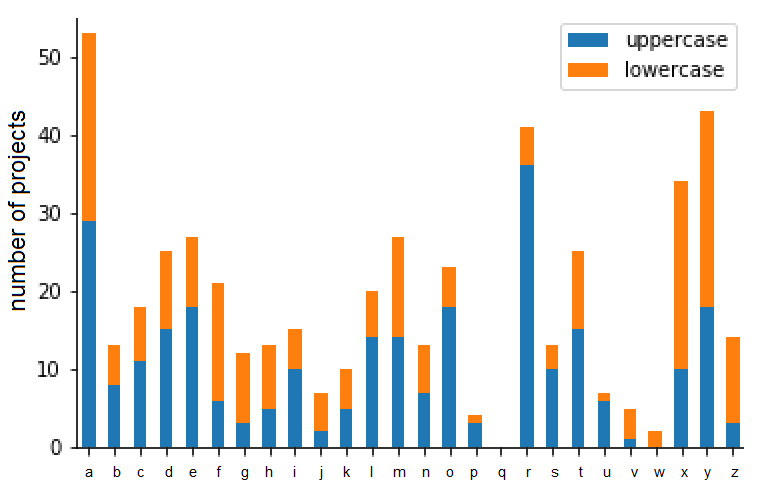
\includegraphics[width=0.95\columnwidth]{fig/project/single_letter_proc}
		\caption{A histogram of single-letter procedures occurrences in Scratch projects}
		\label{fig:one_letter_occurrence_procedures}
	\end{center}
\end{figure} 

%Types analysis
\subsubsection{Types}
\label{res:types}

In the paper of Beniamini et al.~\cite{Beniamini} the authors observe that some letters are highly associated with the data type starting with the same letter: e.g., char for $c$ and string for $s$. They also highlight that the integer data type is a common association for many other letters. Furthermore, a survey for developers showed that variable names $x$, $y$ and $z$ are commonly interpreted as coordinates, and for these letter it seems a balance exists between integer and float associations. 
\begin{figure}[h]
	\begin{center}
		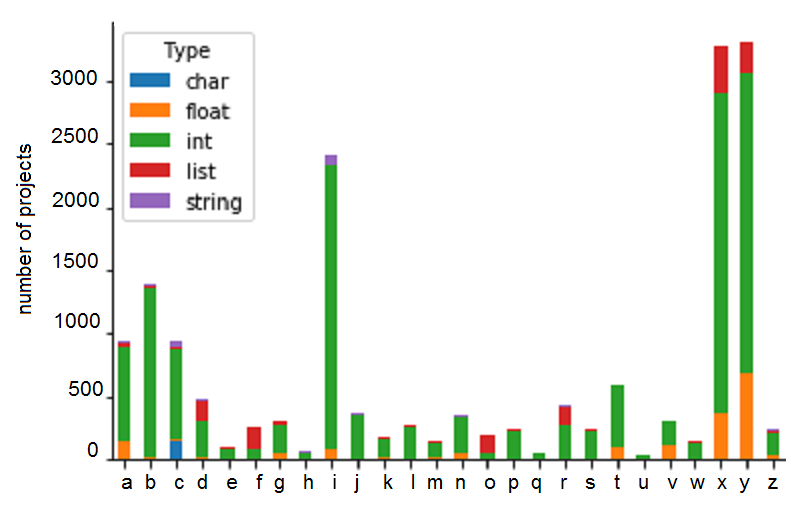
\includegraphics[width=0.95\columnwidth]{fig/project/one_letter_type_double}
		\caption{Inferred types for variables of one letter}
		\label{fig:one_letter_type}
	\end{center}
\end{figure} 

As explained in Section~\ref{sec:design} we conduct a conceptual replication by considering the types of variables as they are used, as opposed to types as guesses by programmers.
%With this process we can compare our results to the types of Beniamini et al.~\cite{Beniamini}. 
Figure~\ref{fig:one_letter_type} shows the distribution of single-letter variables with the types inferred. 
The majority of single-letter variables are encountered as integers in the Scratch dataset. This partially agrees with their \emph{Observation} of integers being common for many letters, however, the data types  are less diverse in Scratch compared to the five programming languages considered.
One \emph{Observation} that contradicts \emph{Observation}s in the original study is related to the string data type. While string data type in the five programming languages studied is commonly associated with $s$ and less frequently with many other letters, the strings are almost completely absent in the Scratch dataset apart from $i$. This is also observed in the other data types where no noticeable usage could be observed for floats, lists or strings. The only exception to some extent is the variable $c$ where we observe some usage linked with the $char$ data type. 
Finally, the presence of floats as types for $x$, $y$ and to lesser extent $z$ seems to support the \emph{Observation} that these single-letters variables are perceived as coordinates suggested by Beniamini et al.~\cite{Beniamini}.

\subsection{Scratch-specific Constructs}
\label{res:Scratch:specific}
In this section we analyze the occurrence of naming practices that are allowed in Scratch, but are missing from or are not common in most mainstream textual languages.
\subsubsection{Spaces in Variable Names}
Most textual programming languages do not allow spaces in variable names. 
FORTRAN ignored spaces, so one could use a space, however that would mean that `apples' and `app les' refer to the same variable. Other languages supporting spaces in variable names are SQL and some Scheme implementations. 
Even languages targeting data analysts rather than software developers recommend spaces to be avoided~\cite{Bochud}.
\begin{figure}
	\begin{center}
		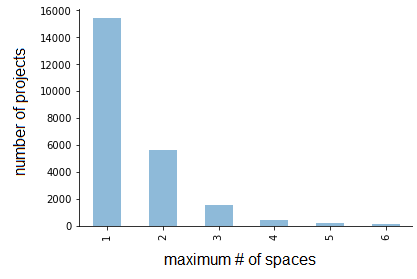
\includegraphics[width=0.8\columnwidth]{fig/project/space_final}
		\caption{Number of spaces in variable names}
		\label{fig:number_of_spaces}
	\end{center}
\end{figure} 
To understand the usage of spaces in variable names, we measure their presence across the unique variable names, and across projects. Out of 67,286 unique variable names in the dataset, we find that 44.05\% have at least one space --30.95\% have one space, 9.91\% have two and 2.15\% have three space characters. For the usage of space character per project, we count the maximum count of a space character in the project's variable names. Out of 69,045 projects which include variables, we find 34\% include variables names with at least one space character. As Fig.~\ref{fig:number_of_spaces} shows variable names with one space character is the most prevalent. 
We conclude that Scratch programmers prefer natural language naming of a variable: the use of a space character in variable names is common to some extent for many users, indicated by the project count, and for many used variable names. 

\begin{figure}[h]
	\begin{center}
		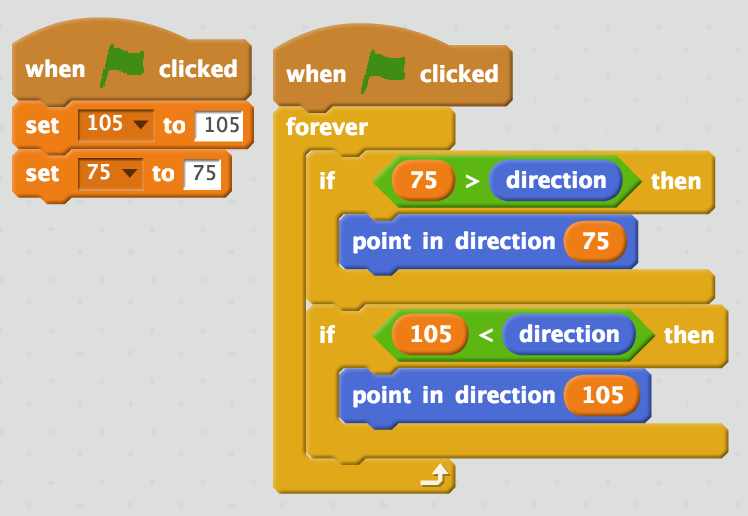
\includegraphics[scale=0.46]{fig/constants}
		\caption{Numeric variable used as a constant}
		\label{fig:constants}
	\end{center}
\end{figure} 	

\subsubsection{Use of Numeric Variable Names}
In addition to spaces in variable names, Scratch even allows the use of numbers and even floating point numbers as variables. We found 718 projects using integer variable names and 19 with floating point names. While their use is rare, we manually examined some projects and numbers are used in interesting and clever ways. 
\begin{figure}[h]
	\begin{center}
		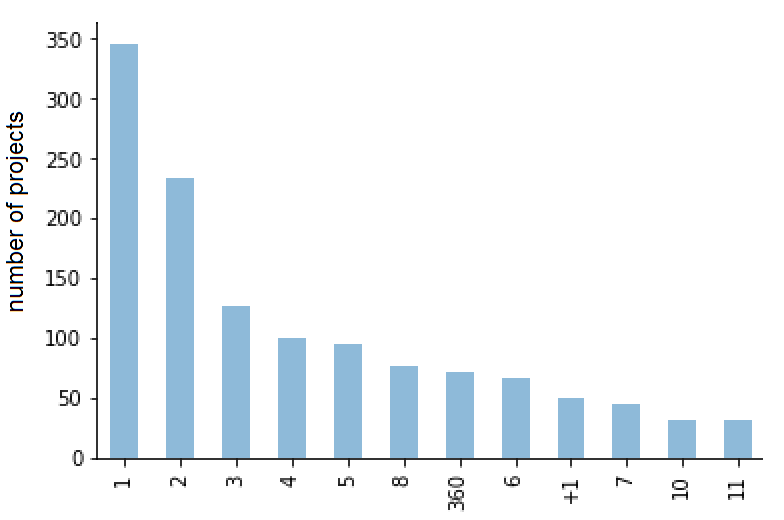
\includegraphics[scale=0.6]{fig/project/numeric}
		\caption{The most popular numeric values used as variables}
		\label{fig:numeric}
	\end{center}
\end{figure} 
The most popular numeric values used as variable names include small natural numbers (1--12) and 360 likely to represent 360$^\circ$ (cf. Fig.~\ref{fig:numeric}).

There seem to be two main uses of numeric variable names. First, some variables with numeric names represent constants, as shown in Fig.~\ref{fig:constants}. This seems to indicate the Scratch programmers prefer to drag in a constant rather than repeatedly type it.

A second use is the use of integer variables as simple list structures. For example, one of the projects we analyzed is a tic-tac-toe game. In that project, the programmer defined nine variables named 1 to 9. Each variable represents one of the nine boxes. Scratch supports lists, so the user here could have also used a list of 9 items, however, they did not. Maybe because they were not familiar with the concept of lists, or maybe they thought this would be easier for the user to memorize the game logic.  

\subsubsection{Use of Textual Labels between Parameters}
Scratch is influenced by the SmallTalk family of languages which is visible form the fact that Scratch allows users to insert textual labels in between parameters in order to make procedures more readable, as shown in Fig.~\ref{fig:procedures}.
This practice seems particular idiomatic to Scratch, since built-in Scratch blocks use a similar syntax, e.g., in the ``say ... for ... seconds" block. 
\begin{figure}
	\begin{center}
		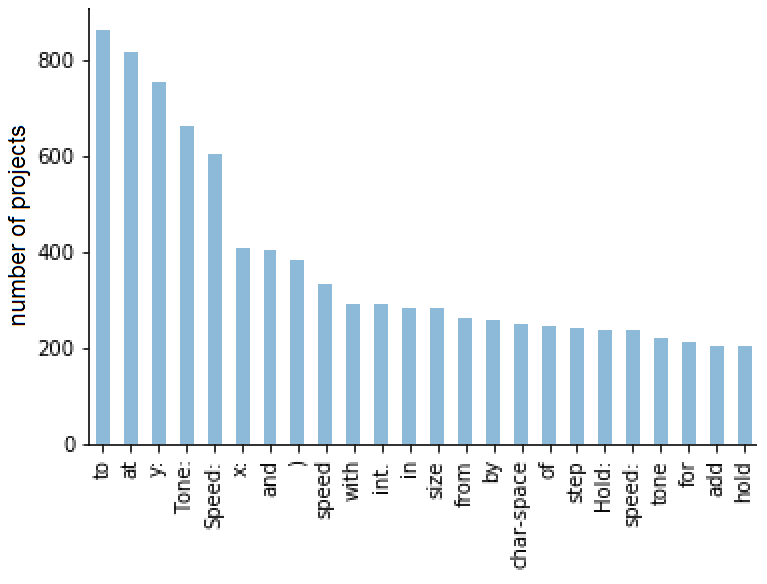
\includegraphics[width=\columnwidth]{fig/project/labels_in_procedures}
		\caption{The most used textual labels in between parameters of procedures}
		\label{fig:labels}
	\end{center}
\end{figure} 
In total 4,415 projects use textual labels, so their use is relatively uncommon. We do however find some interesting patterns. 
Figure~\ref{fig:labels} shows the most commonly used labels. Here we see some patterns common in textual languages, like the use of labels for the names of the parameters `x:' and `y:', and the use of a closing bracket. We suspect the lack of the opening bracket $($ to be caused by the fact that it would be included in the procedure name.
% the names of the parameters `x:' and `y:' 
Furthermore we see the use of `:' at the end of many patterns, which could come from the users being inspired by Scratch default blocks, which use the colon as shown in Fig.~\ref{fig:xy_Scratchblocks}. 
Finally the use of the space (char-space in Fig.~\ref{fig:labels}) is interesting, since Scratch already leaves some room between the parameters, also when a space is not used. 
%The use of space as a separator could indicate that Scratch users feel room between variables is currently too small.

\section{Threats to Validity}
As any empirical study our work is subject to series of threats to validity.
Construct validity of our study might be threatened by the operationalization of the notion of a type. 
Due to the lack of explicit type declaration in Scratch our approach inferred the type by inspecting the value assigned to the variable. To be representative for a project, our method counted the different types encountered for the same variable within a project. For example if the variable ``score" was set to ``empty" at first, and then set to 0 in a different script, we count two types for the variable: one string and one integer. The same can be applied in textual languages with less strict type systems such as PHP. While the method is simple, it assures that data types used by Scratch programmers are represented in the data, and forms a good proxy to compare the results to the perceptions of professional developers. It is possible that these data types do not reflect the perception of users precisely. This why this threat will be addressed in future work by surveying students in our running Scratch MOOC.

Another threat to the construct validity is our decision of what is a variable name in Scratch. We choose to include the names of variables created specifically through ``Make a Variable" button in Scratch UI. A possible threat is that this approach does not represent other types of variables in a Scratch programs. Sprites for example can be named, thus considered as variables. However, we believe they should be excluded from our study, since we perform a dependent replication study to variable names in textual languages. Therefore what we consider as a Scratch variable must hold a major property similar to variables in the textual languages: its name must be entered by the user. In Scratch, however, sprites are assigned default names automatically, and they often remain unchanged by the users~\cite{MoreonoRobles}.

One threat to the internal validity of our study comes from the use of non-Latin characters in identifiers. These characters are encoded as series of question marks, which is a limitation we inherit from the original dataset. Since one non-Latin character can be encoded as several question marks, the variable/procedure names length reported would overestimate the actual length. However, the impact of these identifiers is limited as the majority of Scratch programmers are from countries that use Latin alphabet\footnote{\url{https://scratch.mit.edu/statistics/}}. To validate this, we manually analyzed the variable names extracted and found that merely 450 variables have non-Latin alphabetic characters, less than 0.67\% of the total 67,287 unique variable names. Therefore, we did not exclude names with non-Latin characters from the analysis.

Finally, a threat to the external validity concerns the generalization of the study results. We argue that we use a large dataset which comprises around 1\% of 23 million currently shared Scratch projects. It could be that the dataset does not reflect the users trend for identifier naming. However, the Scratch community represents novice programmers with younger age. For this type of users, it is difficult to imaging they have an established trend in naming without prior education.

\section{Conclusion}
In this paper, we study naming patterns for variables and procedures in the Scratch programming language, a block-based programming language aimed at novice programmers. We use a previously released dataset consisting of 250,000 Scratch programs. 

Our analysis shows that Scratch programmers most often use variable names between 4 and 10 characters in length, while procedure names in Scratch tend to have longer names than the variables. For the single-letter variables, the most commonly used names are \emph{x}, \emph{y} and \emph{i}. When compared to the other programming languages, Scratch variable length distribution, and the usage of single uppercase letters seems to be similar to the pattern found in Perl, while for the lowercase letters---to the pattern found in Java. Spaces in variable names, a feature relatively unique to Scratch, are used in 34\% of projects in which variables can be found. The usage of textual string between parameters appears as not so common, however textual patterns used imply an inference from textual languages by using brackets for example.

The paper makes the following contributions:
\begin{itemize}
\item A detailed analysis of variables name length and single-letter variables in particular, replicating \cite{Beniamini} on the Scratch programming language
\item An analysis of procedure names in Scratch
\item An analysis of naming patterns unique to Scratch, including spaces in variable names, numeric variable names and textual labels in procedures.
\end{itemize}

We believe the naming patterns found in our study give an indication that Scratch programmers may incur difficulties when transiting to the use of mainstream textual programming languages. Those languages restrict the use of spaces in identifiers and more often divert into short and single-letter names---tendencies opposite to the naming preferences in Scratch.

This paper gives rise to a number of directions for future work. Firstly, Beniamini et al.~\cite{Beniamini} included a survey in which they ask developers to predict the type of a (one letter) variable. It could be interesting to ask a similar question to Scratch programmers for common variable names. Furthermore, a detailed study into the readability of variable names with and without spaces, and procedures with and without labels would help us to create naming guidelines for Scratch. Finally, one additional area to explore is the relation between name length of variables with the level of computational thinking of the Scratch programmer in addition to other demographic factors like gender, age and language.  

% trigger a \newpage just before the given reference
% number - used to balance the columns on the last page
% adjust value as needed - may need to be readjusted if
% the document is modified later
%\IEEEtriggeratref{8}
% The "triggered" command can be changed if desired:
%\IEEEtriggercmd{\enlargethispage{-5in}}

% references section
\balance
% can use a bibliography generated by BibTeX as a .bbl file
% BibTeX documentation can be easily obtained at:
% http://mirror.ctan.org/biblio/bibtex/contrib/doc/
% The IEEEtran BibTeX style support page is at:
% http://www.michaelshell.org/tex/ieeetran/bibtex/

\bibliographystyle{IEEEtran}
% argument is your BibTeX string definitions and bibliography database(s)
\bibliography{paper_final}
%
% <OR> manually copy in the resultant .bbl file
% set second argument of \begin to the number of references
% (used to reserve space for the reference number labels box)

% that's all folks
\end{document}


